\begin{enumerate}
	\item Exercício
	
	Esboçe a região de integração e o sólido cujo volume é dado pela integral abaixo: 
	$$\integral_0^1 \integral_0^1 \left(4 - x - 2y\right)\, dx dy$$
	
	\begin{figure}[H]
		\caption{Integrais duplas - Aula 9 - Exercício I}
		\label{v09_a09_e01}
		\centering
		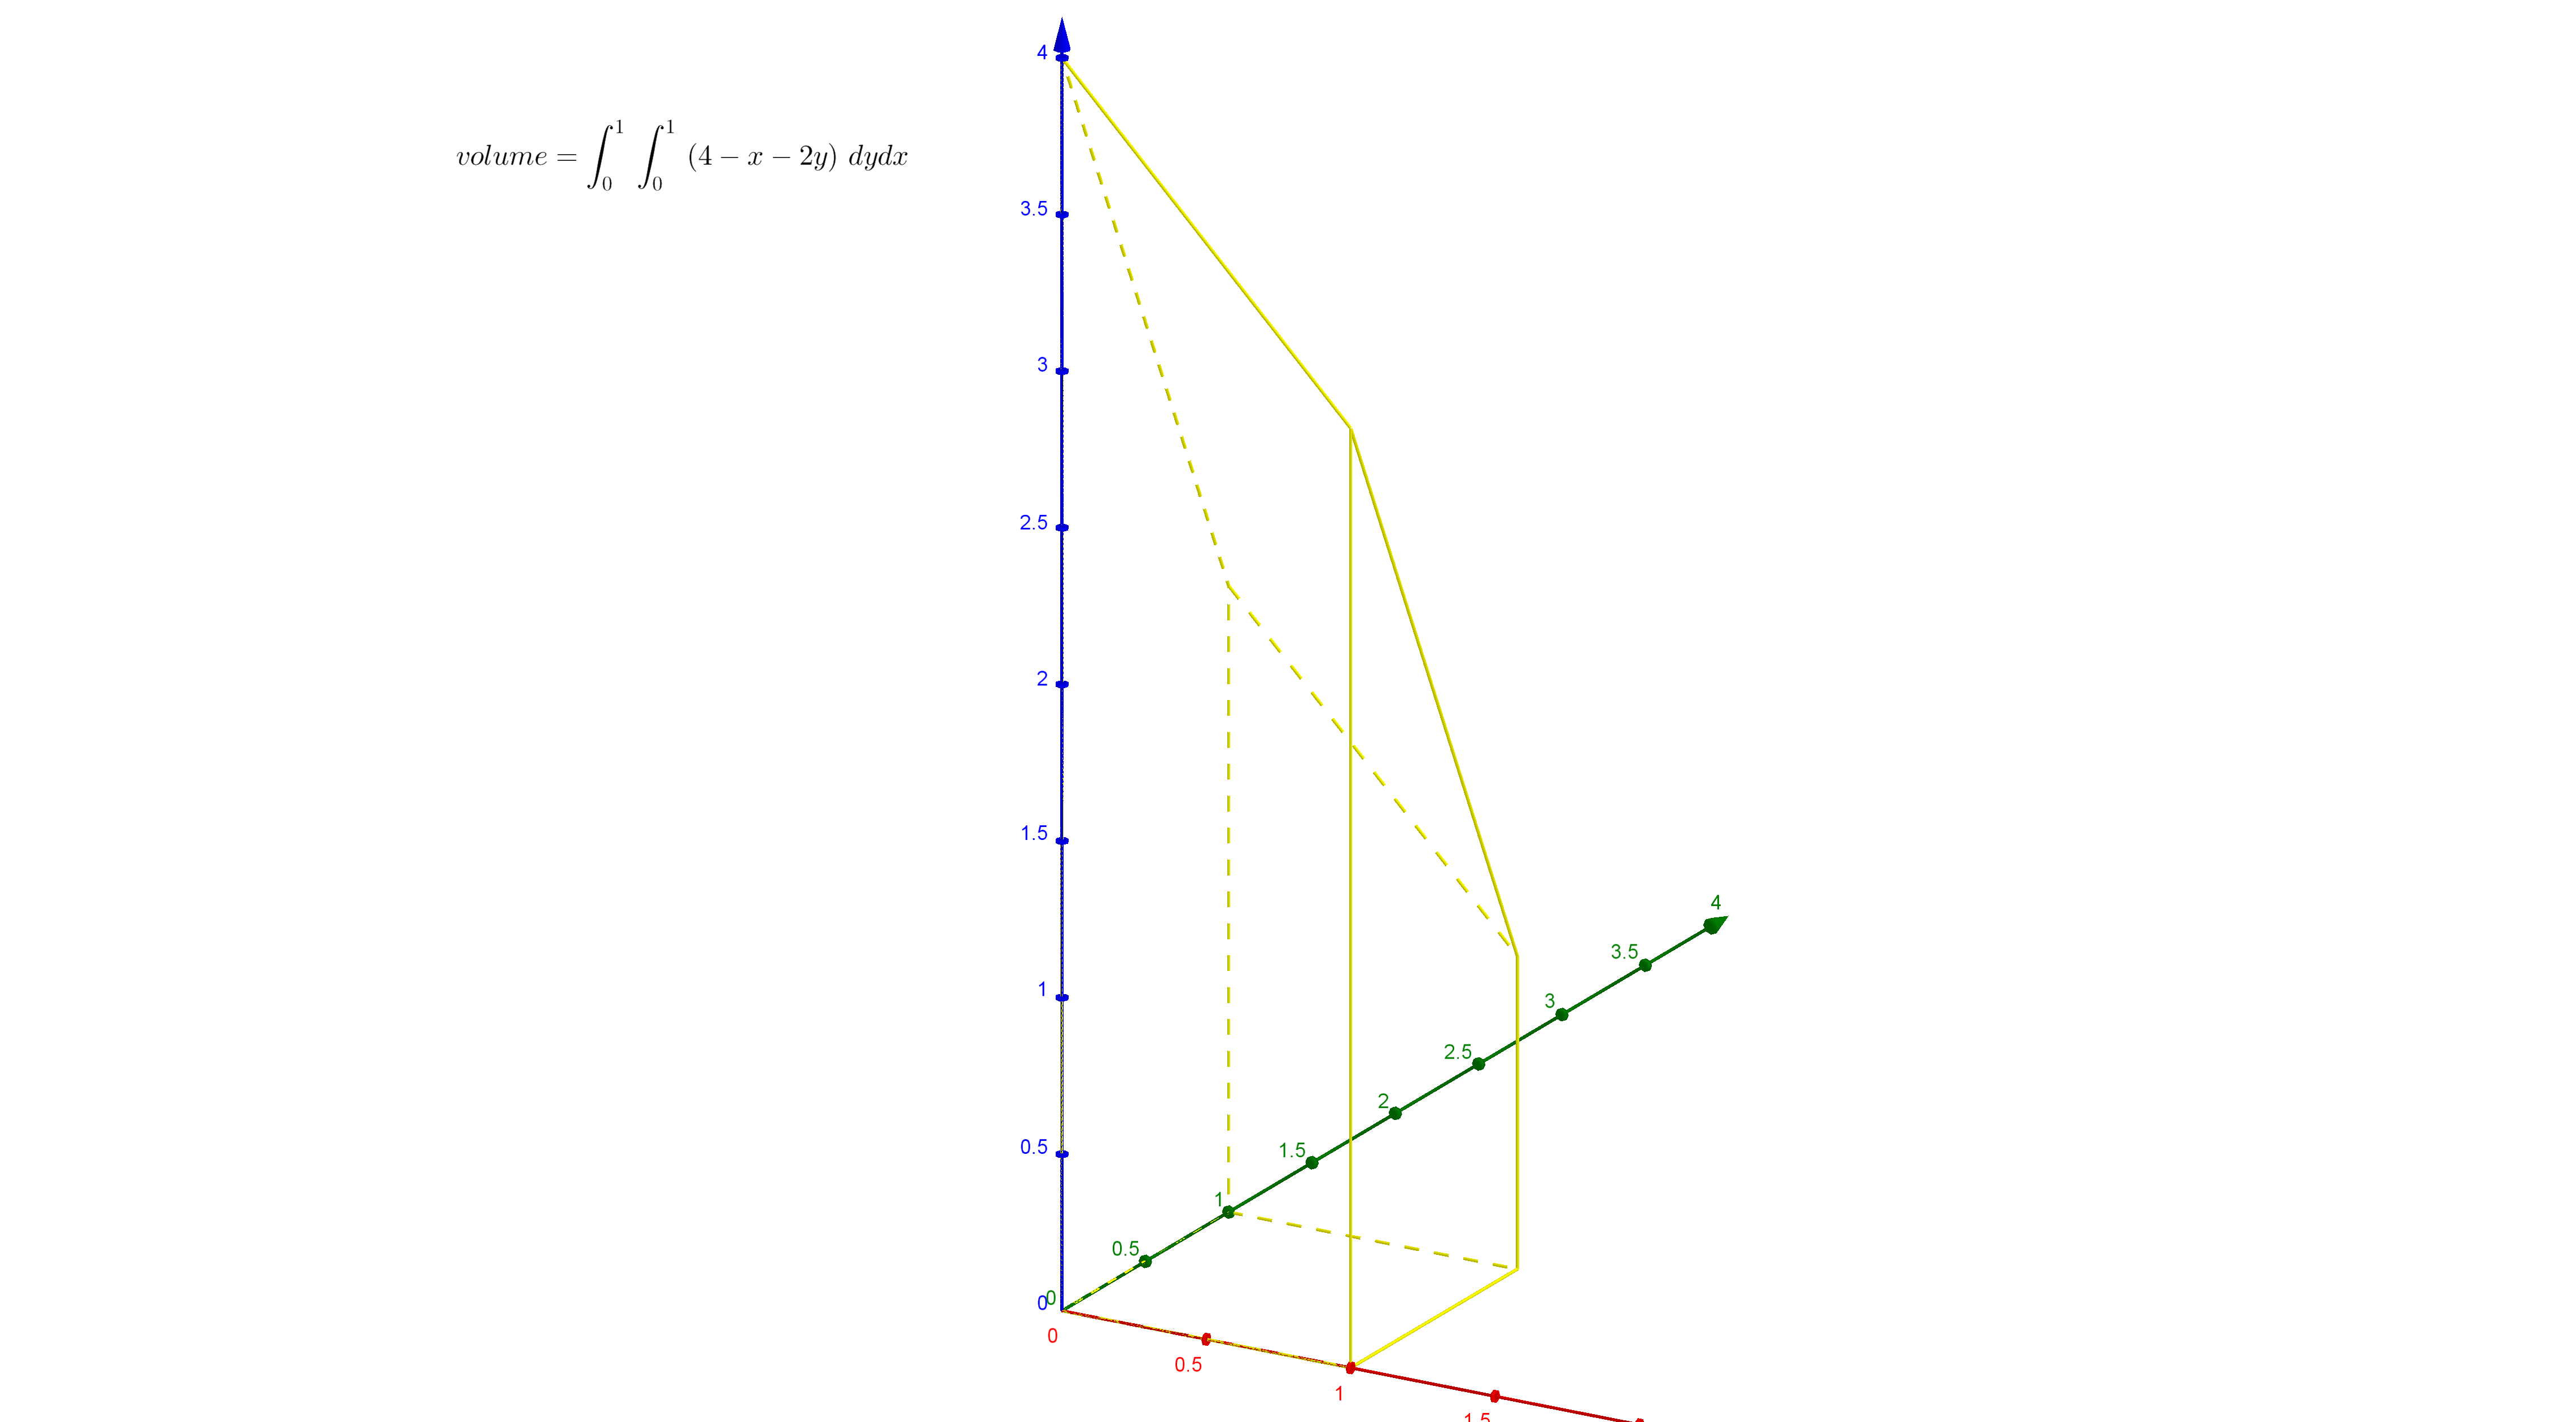
\includegraphics[width=\textwidth]{v09_a09_e01.png}		
	\end{figure}
	
	$v = \integral_0^1 \integral_0^1 \left(4 - x - 2y\right)\, dx dy = \integral_0^1 dx \left(4\integral_0^1 dy - x\integral_0^1 dy - 2\integral_0^1 y\, dy\right) = 4\integral_0^1 dx \integral_0^1 dy - \integral_0^1 x\, dx \integral_0^1 dy - 2\integral_0^1 dx \integral_0^1 y\, dy = 4[x]_0^1 [y]_0^1 - \left[\dfrac{x^2}{2}\right]_0^1 [y]_0^1 - 2[x]_0^1 \left[\dfrac{y^2}{2}\right]_0^1 = 4 - \dfrac{1}{2} - \overstrike{2}\dfrac{1}{\overstrike{2}} = \frac{8 - 1 - 2}{2} = \dfrac{5}{2} = 2,5$	
\end{enumerate}